\chapter {TINJAUAN PUSTAKA}
Bab ini membahas mengenai teori-teori dasar yang digunakan dalam Tugas Akhir. Teori-teori tersebut diantaranya adalah \textit{Transfer Learning}, \textit{Server} dan beberapa teori lain yang mendukung pembuatan Tugas Akhir. Penjelasan ini bertujuan untuk memberikan gambaran umum dan diharapkan dapat mendukung sistem yang dibangun.

\section{Android}
Android menyediakan kerangka kerja aplikasi yang kaya dan memungkinkan Anda membangun aplikasi dan game inovatif untuk perangkat seluler di lingkungan bahasa pemrograman Java.   Android merupakan sistem operasi perangkat bergerak yang berbasis linux kernel dan merupakan open-source. Android dikembangkan oleh Google.

\par Perangkat keras yang mendukung Android terutama didasarkan pada platform arsitektur ARM. Ada sekitar 2,6 juta aplikasi yang dikembangkan untuk Android. Android mengandalkan Linux versi 2.6 untuk layanan sistem inti seperti keamanan, manajemen memori, manajemen proses, tumpukan jaringan, dan model driver. 

\par Komponen-komponen dalam platform Android antara lain : linux kernel, lapisan abstraksi perangkat keras, native c++ dan \textit{android runtime}, kerangka kerja Java API, dan sistem aplikasi \cite{android_def}.


\section{Transfer Learning}
\par Transfer Learning adalah sebuah riset masalah pada pembelajaran mesin yang terfokus pada menyimpan pengetahuan yang didapat ketika menyelesaikan suatu masalah dan mengaplikasikannya ke masalah yang berbeda namun berhubungan \cite{transfer_def}. Transfer Learning akan berfungsi dengan baik apabila fitur-fitur pada permasalahan awal bersifat umum dan bukan spesifik sehingga model yang dihasilkan dapat digunakan kembali pada permasalahan yang sejenis.
\begin{figure}[!ht]
	\centering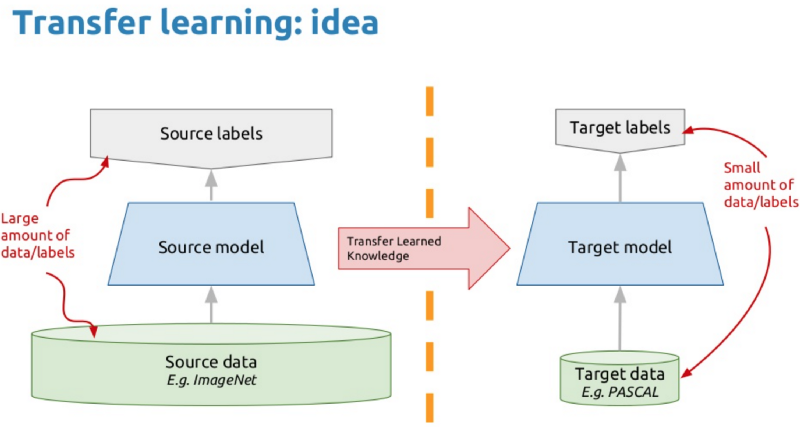
\includegraphics[width=0.8\textwidth]{bab2/figures/transfer-works.png}
	\caption{Diagram alir transfer learning\cite{transfer_pic}}
	\label{fig:transfer-works}
\end{figure}
\par Pendekatan Transfer Learning adalah dengan tiga metode, yaitu : 

\subsection{Melatih Sebuah Model untuk Menggunakannya Kembali}
\par Ketika kita ingin menyelesaikan Task A namun tidak memiliki cukup data untuk melatihnya dengan Deep Neural Network. Di sisi lain kita memiliki Task B dimana kita bisa melatihnya dengan Deep Neural Network. Maka kita dapat melatih Task B dengan Deep Neural Network dan menggunakannya sebagai titik awal dalam menyelesaikan Task A.

\subsection{Menggunakan Pre-Trained Model}
\par Pendekatan kedua adalah menggunakan dengan menggunakan pre-trained model atau model yang telah dilatih sebelumnya. Di internet banyak yang menyediakan pre-trained model ini, salah satunya Keras. Keras merupakan sebuah library pada Python yang menyediakan berbagai pre-trained model seperti VGG16, VGG19, XCeption, MobileNet dan lain-lain. 

\subsection{Ekstraksi Fitur}
\par Pendekatan lain adalah menggunakan algoritma \textit{Deep Learning} untuk menemukan representasi terbaik dari permasalahan. Pendekatan ini sering juga disebut \textit{Representation Learning}.  Cara menggunakan pendekatan ini adalah dengan menemukan fitur apa saja yang paling menggambarkan permasalahan kita. 
\par Meskipun metode Deep Learning dapat mengekstrak fitur secara otomatis, kita harus menentukan fitur mana saja yang ingin dimasukkan dalam \textit{Network}. Representasi yang sudah dipelajari kemudian dapat digunakan untuk menyelesaikan permasalahan lain juga. Metode ini cocok untuk menyelesaikan permasalahan Visi Komputer karena dapat mengurangi ukuran data set yang kemudian mengurangi waktu komputasi juga\cite{transfer_how}.

\begin{figure}[ht]
	\centering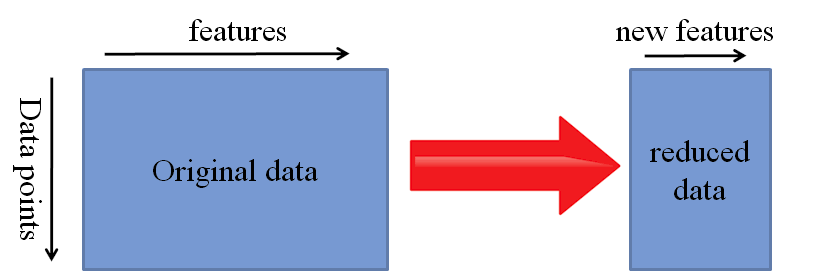
\includegraphics[width=0.7\textwidth]{bab2/figures/rep_features.png}
	\caption{Pembelajaran Representasi\cite{transfer_how}}
	\label{fig:rep-works}
\end{figure}

\section{Server}
\par Server dapat merujuk baik pada perangkat keras atau perangkat lunak yang menyediakan layanan tertentu kepada pengguna. Jika merujuk pada perangkat keras, server digunakan untuk menyimpan semua data. Sedangkan pada sisi perangkat lunak, fungsi server adalah sebagai pusat kontrol untuk memproses permintaan yang diterima dari browser.

\par Secara sederhana, server bekerja atas permintaan dari sebuah klien. Misalnya saja untuk kasus web server, ketika Anda mengetikkan suatu alamat website menggunakan browser, maka artinya komputer Anda sedang bertindak sebagai klien yang meminta informasi kepada web server. Web server tersebut kemudian mengirimkan isi website ke komputer Anda, sehingga Anda pun dapat mengakses isi website tersebut.

\par Untuk kasus lainnya, seperti server FTP, mungkin agak sedikit berbeda. Pada server FTP, Anda dapat mengunggah sebuah dokumen atau data menuju server FTP, sehingga dapat disimpan dalam server tersebut. Sebagai klien, Anda berhak untuk menyimpan data Anda di server FTP. Nantinya, jika ada orang lain yang tergabung dalam jaringan server tersebut dan ingin mengunduh data atau dokumen Anda, maka server FTP akan menyediakan koneksi untuk klien lain tersebut.

\par Sebuah perangkat komputer yang dijadikan server biasanya dirancang sedikit berbeda dari komputer – komputer klien. Dalam hal spesifikasi perangkat dan juga dalam hal sistem operasi misalnya, spesifikasi perangkat komputer yang digunakan sebagai server harus dibuat tinggi (karena harus menangani lalu lintas data yang cukup besar), sedangkan sistem operasinya harus menggunakan sistem operasi khusus server seperti Windows Server atau pun Linux Ubuntu Server / Linux Mint Server\cite{server_def}.

\section{Python}
\par Python adalah bahasa pemrograman yang populer. Python sering dimanfaatkan dalam pengembangan web, perangkat lunak, penelitian, dan system scripting. Python dapat digunakan untuk menangani data besar dan melakukan operasi matematika yang kompleks. Python bekerja di berbagai platform seperti Windows, Mac, Linux, Raspberry Pi, dan lain-lain. Python dirancang untuk mudah dibaca, yaitu memiliki sintaks yang sederhana dan
menggunakan bahasa Inggris\cite{python_def}.
Penulis menggunakan Python dalam Tugas Akhir ini karena tersedianya library pembelajaran mesin dan pembelajaran dalam yang lengkap pada bahasa pemrograman ini.


\section{Tensorflow}
\par TensorFlow adalah library \textit{open source} untuk pembuatan program yang membutuhkan komputasi numerik berkinerja tinggi. Dibuat oleh tim Google Brain, TensorFlow adalah librari \textit{open-source} untuk komputasi numerik dan pembelajaran mesin skala besar. Tensorflow menggunakan Python untuk menyediakan API front-end yang nyaman untuk membangun aplikasi dengan kerangka kerja, sambil mengeksekusi aplikasi tersebut dalam C++.TensorFlow menyediakan fungsi-fungsi \textit{machine learning} dan \textit{deep learning}, dan dapat dijalankan dalam CPU atau GPU\cite{tensorflow_def}.

\section{Keras}
\par Keras adalah API \textit{neural network} tingkat tinggi, ditulis dengan Python dan mampu berjalan di atas TensorFlow, CNTK, atau Theano. Keras dikembangkan dengan fokus pada mempercepat eksperimen\cite{keras_def}.
\par Keras tidak melakukan operasi tingkat rendahnya sendiri, seperti produk tensor dan konvolusi. Keras bergantung pada back-end. Meskipun Keras mendukung beberapa back-end, back-end utamanya adalah TensorFlow, dan pendukung utamanya adalah Google. 
\par Keras API dikemas dalam TensorFlow sebagai tf.keras, yang seperti yang disebutkan sebelumnya akan menjadi TensorFlow API utama pada TensorFlow 2.0.

\section{ImageNet}
\par ImageNet adalah sebuah proyek yang bertujuan untuk memberi label dan mengkategorikan gambar ke dalam 22.000 kategori objek berbeda untuk riset Visi Komputer. Model-model dilatih pada lebih dari 1,2 juta gambar untuk pelatihan dengan 50.000 gambar validasi dan 100.000 gambar uji\cite{vgg19_def}.

\section{VGG16} 
\par VGG16 (juga disebut OxfordNet) adalah arsitektur jaringan saraf convolutional yang dinamai Grup Visual Geometry dari Oxford, yang mengembangkannya.VGG16 terdiri dari 3 x 3 layer konvolusi, 2 x 2 max layer, dan fully-connected layer. Total layer pada VGG16 adalah 16\cite{vgg16_def}.

\par Untuk menghitung layer konvolusi, matriks 3x3 pada input data gambar dibaca dari kiri atas ke kanan bawah. 
Pada setiap posisi gambar, dihasilkan sebuah angka yang merupakan dot product antara bagian gambar tersebut dengan filter yang digunakan. Dengan menggeser \textit{(convolve)} filter di setiap kemungkinan posisi filter pada gambar, dihasilkan sebuah activation map.

\par Proses ini diulang dengan beberapa filter berbeda, hingga menghasilkan “gambar” baru yang merupakan kumpulan dari activation maps.

\par Pooling layer adalah lapisan yang mengurangi dimensi dari feature map atau lebih dikenal dengan langkan untuk downsampling, sehingga mempercepat komputasi karena parameter yang harus diupdate semakin sedikit dan mengatasi overfitting. Pooling yang biasa digunakan adalah Max Pooling dan Average Pooling. Max Pooling untuk menentukan nilai maksimum tiap pergeseran filter, sementara Average Pooling akan menentukan nilai rata-ratanya.
\begin{figure}[!ht]
	\centering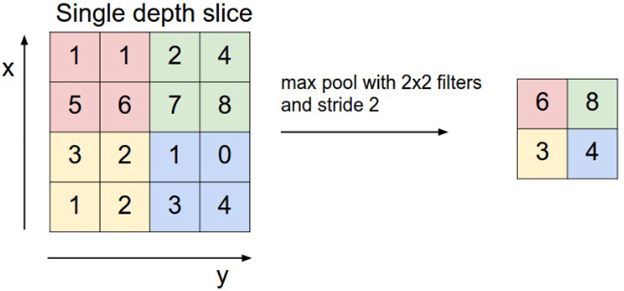
\includegraphics[width=0.7\textwidth]{bab2/figures/max pooling.png}
	\caption{Contoh dari Max Pooling\cite{max_pool}}
	\label{fig:abstraksi1}
\end{figure}


\section{VGG19}
\par VGG-19 adalah jaringan saraf convolutional yang dilatih pada lebih dari satu juta gambar dari database ImageNet. Jaringan ini memiliki 19 lapisan dan dapat mengklasifikasikan gambar ke dalam 1000 kategori objek, seperti keyboard, mouse, pensil, dan banyak binatang. Akibatnya, jaringan telah mempelajari representasi fitur yang kaya untuk berbagai gambar. Jaringan memiliki ukuran input gambar 224 x 224\cite{imagenet_def}.
\begin{figure}[!ht]
	\centering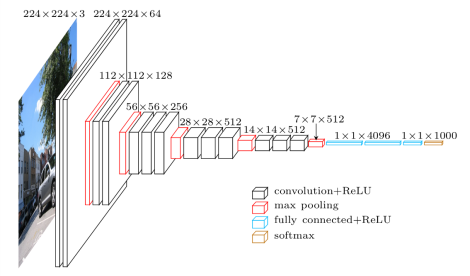
\includegraphics[width=0.7\textwidth]{bab2/figures/figure-vgg.png}
	\caption{Visualisasi dari arsitektur VGG\cite{figure_vgg}}
	\label{fig:abstraksi1}
\end{figure}

\par Kelebihan VGG16 dan VGG19 antara lain jumlah layernya yang dapat dianggap \textit{deep}, relatif mudah untuk dijelaskan dibanding arsitektur lain. Kekurangan dari VGG16 dan VGG19 yaitu sangat lama untuk proses pelatihan,dan ukuran yang sangat besar yaitu 533 MB untuk VGG16 dan 574 MB untuk VGG19.


\section{MobileNet}
\par MobileNet didasarkan pada arsitektur ramping yang menggunakan konvolusi \textit{depth-wise} terpisah untuk membangun jaringan saraf yang dalam dan ringan\cite{mobilenet_def}. Keunggulan dari MobileNet adalah kompleksitas yang lebih kecil dan ukuran yang lebih kecil juga. Dengan kompleksitas yang lebih kecil, kekurangan dari MobileNet adalah akurasinya yang tidak setinggi arsitektur yang lebih kompleks. Berikut ini adalah gambar dari cara kerja \textit{depth-wise separable convolution} pada MobileNet.

\begin{figure}[!ht]
	\centering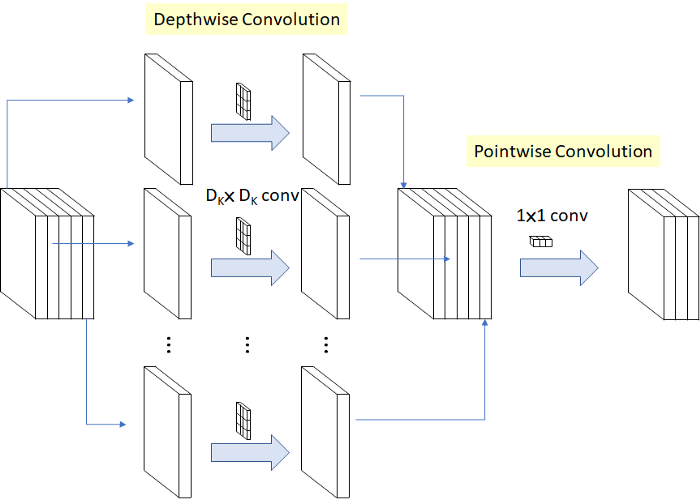
\includegraphics[width=0.7\textwidth]{bab2/figures/mobilenet.png}
	\caption{\textit{Depth-Wise Separable Convolution pada MobileNet}\cite{mobilenet_def}}
	\label{fig:abstraksi1}
\end{figure}

\section{ResNet50}
\par ResNet adalah singkatan dari Residual Network. Residual dapat dipahami sebagai pengurangan fitur yang dipelajari dari input layer tersebut\cite{resnet_def}. Karena hal ini, ResNet merupakan arsitektur yang dalam dengan jumlah layer mencapai 200. ResNet yang akan dipakai oleh penulis adalah ResNet50, yang berarti Residual Network dengan jumlah layer 50. Meskipun jumlah layer pada ResNet lebih banyak daripada VGG16 atau VGG19, ukuran modelnya lebih kecil karena penggunaan pooling global rata-rata dan bukan fully-connected layer. Ukuran ResNet50 adalah 102 MB.

\section{InceptionV3}
\par Tujuan dari modul Inception adalah untuk bertindak sebagai "ekstraktor fitur multi-level" dengan menghitung konvolusi 1×1, 3×3, dan 5×5 dalam modul jaringan yang sama - output dari filter ini kemudian ditumpuk bersama dimensi channel dan dimasukkan ke lapisan berikutnya dalam jaringan.

\par Inkarnasi asli dari arsitektur ini disebut GoogLeNet, tetapi manifestasi selanjutnya hanya disebut Inception vN di mana N mengacu pada nomor versi yang dikeluarkan oleh Google.

\par InceptionV3 memiliki 42 layer, namun ukurannya lebih rendah dari VGG, yaitu 96 MB.

\begin{figure}[!ht]
	\centering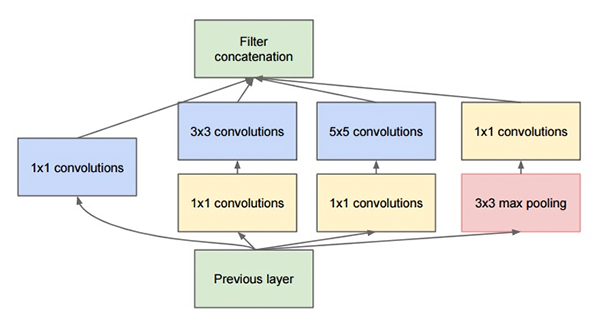
\includegraphics[width=0.7\textwidth]{bab2/figures/inception.png}
	\caption{Inception Model\cite{inception}}
	\label{fig:abstraksi1}
\end{figure}
\section{Xception}
\par Xception diciptakan oleh pembuat dan kepala pengelola Keras yaitu Francois Chollet. Xception sama seperti Inception, hanya saja modul standar Inception digantikan oleh \textit{depth-wise separable convolution}. Keunggulan dari Xception adalah ukuran arsitekturnya yang paling kecil yaitu 91 MB\cite{xception}.


\section{Logistic Regression}
\par Logistic Regression digunakan dalam ilmu biologi pada awal abad kedua puluh. Itu kemudian digunakan dalam banyak aplikasi ilmu sosial. Logistic Regression digunakan ketika target adalah kategorikal.

\begin{figure}[!ht]
	\centering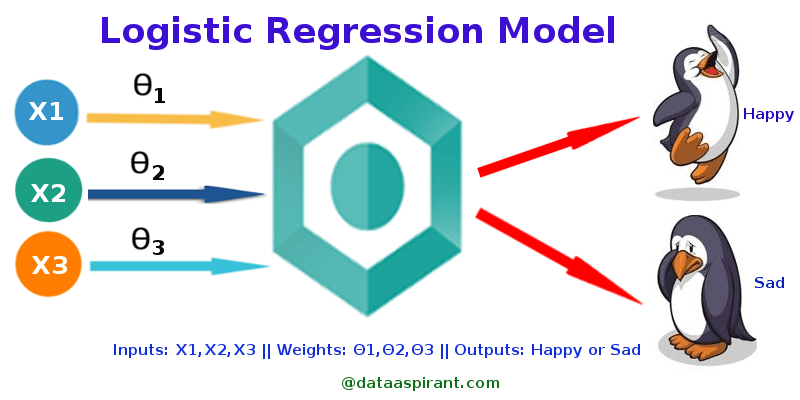
\includegraphics[width=0.9\textwidth]{bab2/figures/logistic.png}
	\caption{Visualisasi dari Logistic Regression\cite{logistic_def}}
	\label{fig:abstraksi1}
\end{figure}
\section{Precision}
\par Precision didefinisikan sebagai jumlah benar positif dibagi dengan jumlah benar positif ditambah jumlah salah positif. Salah positif adalah kasus-kasus yang oleh modelnya salah diberi label sebagai positif yang sebenarnya negatif\cite{precisionrecall}.

\section{Recall}
\par Recall adalah jumlah benar positif dibagi jumlah benar positif dibagi jumlah salah negatif \cite{precisionrecall}. Salah negatif menunjukkan nilai di mana kelas aktual adalah ya tetapi kelas prediksi adalah tidak. Misalnya, jika kelas aktual mengatakan bahwa akan hujan tetapi kelas prediksi menunjukkan bahwa tidak akan ada hujan.

\section{F1 Score}
\par Penghitungan F1 Score adalah dengan cara mengalikan dua dengan precision dan recall kemudian dibagi dengan penjumlahan precision dan recall. F1 Score mungkin merupakan ukuran yang lebih baik untuk digunakan jika kita perlu menemukan keseimbangan antara Precision dan Recall dan ada distribusi kelas yang tidak rata\cite{f1score_def}.

\begin{figure}[!ht]
	\centering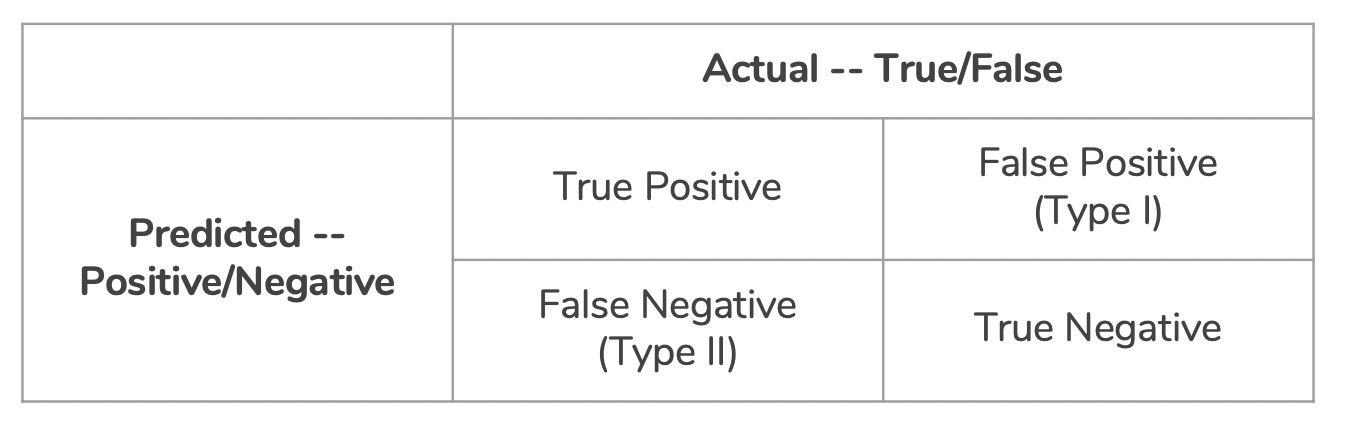
\includegraphics[width=0.9\textwidth]{bab2/figures/confusion.png}
	\caption{\textit{Confusion Matrix}\cite{precisionrecall}}
	\label{fig:conf}
\end{figure}

\begin{figure}[!ht]
	\centering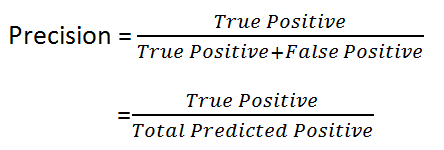
\includegraphics[width=0.7\textwidth]{bab2/figures/precision.png}
	\caption{Rumus\textit{ Precision}\cite{precisionrecall}}
	\label{fig:conf}
\end{figure}

\begin{figure}[!ht]
	\centering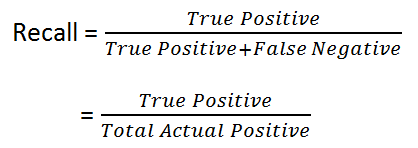
\includegraphics[width=0.7\textwidth]{bab2/figures/recall.png}
	\caption{Rumus\textit{ Recall}\cite{precisionrecall}}
	\label{fig:conf}
\end{figure}

\begin{figure}[!ht]
	\centering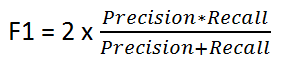
\includegraphics[width=0.7\textwidth]{bab2/figures/f1.png}
	\caption{Rumus \textit{F1 Score}\cite{precisionrecall}}
	\label{fig:conf}
\end{figure}

\section{Spring}
\par Spring adalah sebuah kerangka kerja yang bersifat \textit{open-source}. Spring sendiri pertama kali dibuat oleh Rod Johnson tahun 2002 sebagai alternatif dari Java Enterprise Edition yang bertujuan untuk mengatasi masalah desain sistem dalam pengembangan aplikasi enterprise. Selain itu, Spring juga mengimplementasikan beberapa teknologi IoC (\textit{Inversion of Control}) dan DI (\textit{Dependency Injection}) ke dalam sebuah MVC \textit{(Model View Controller})\cite{spring_def}. 